\section{Introduction}\label{sec:intro}

\begin{figure}[!ht]
    \centering
    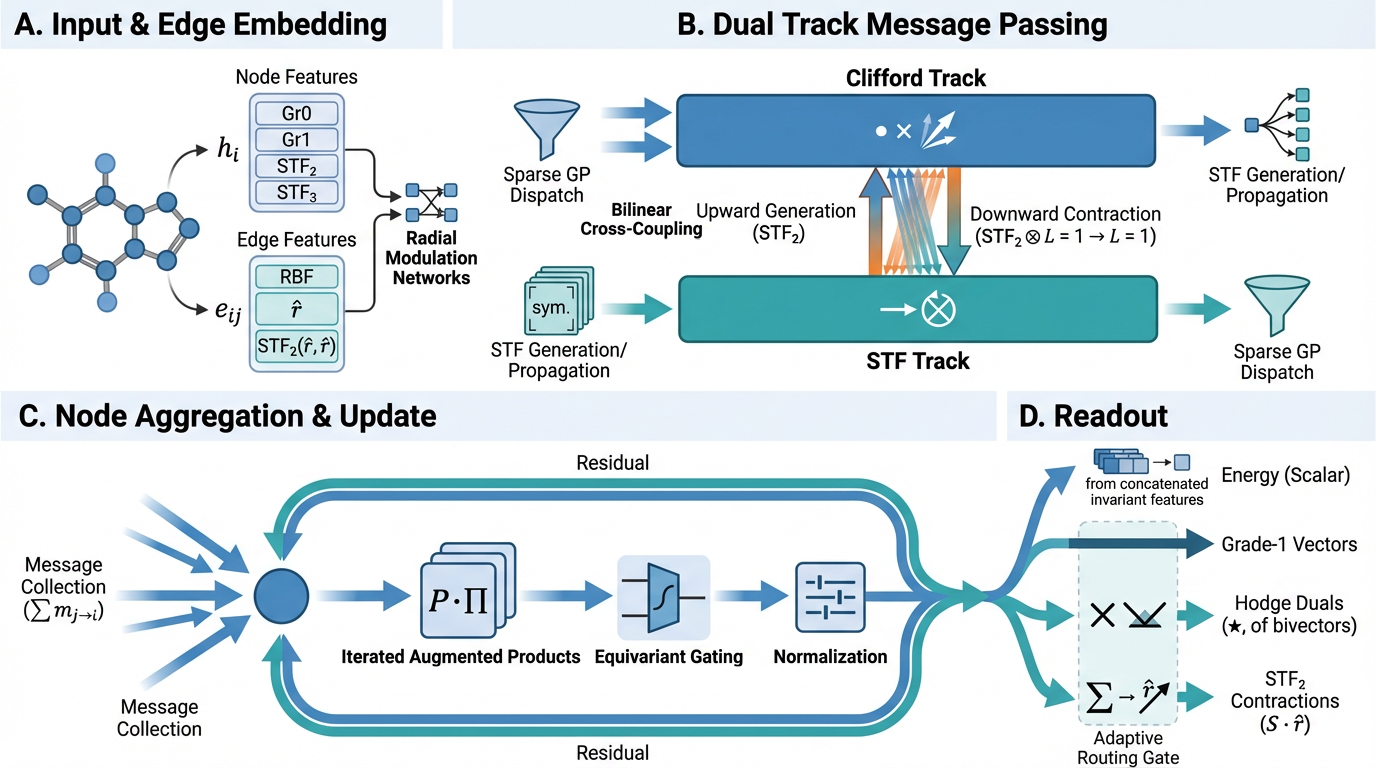
\includegraphics[width=1\linewidth]{resources/cliffordSTFMethod.png}
    \caption{\textbf{Schematic of the CliffordSTF pipeline}. (A) Atoms and edges are embedded with multivector and STF features, including explicit $L{=}2$ edge descriptors. (B) The core message-passing block uses a dual-track design where the Clifford track (geometric products) and STF track are coupled via bilinear generation and contraction operations. (C) Node updates incorporate iterated augmented products for multi-body correlations followed by equivariant gating. (D) Energy and forces are predicted from a combination of invariant and vector sources, including $L{=}2$ contractions ($S \cdot \hat{r}$) that capture angular force components inaccessible to $L \leq 1$ features.}
    \label{fig:architecture}
\end{figure}

Machine learning interatomic potentials (MLIPs) have emerged as practical surrogates for first-principles electronic structure calculations, enabling molecular dynamics at scales inaccessible to density functional theory \citep{unke2021machine}. A central design challenge is encoding the symmetries of physical law: energies must be invariant and forces equivariant under rotations and translations. Force prediction, in particular, decomposes into a magnitude component and a directional component, and directional accuracy governs whether trajectories stay on the correct potential-energy basin even when scalar errors look small. The dominant approach to building such equivariant features constructs them from spherical harmonics composed through tensor products weighted by Clebsch--Gordan (CG) coefficients \citep{thomas2018tensor,batzner2022nequip,batatia2022mace}, but the cost of high-order couplings scales steeply with the maximum angular momentum order $L$, motivating both efficient implementations \citep{geiger2022e3nn,passaro2023escn} and CG-free reformulations based on irreducible Cartesian tensors \citep{simeon2023tensornet,zaverkin2024ictp,wang2024n}.

Clifford (geometric) algebra offers a third route. Architectures in this lineage embed vectors into the eight-dimensional algebra $\mathrm{Cl}(3,0)$ and replace learned tensor products with the single closed-form geometric product, which acts uniformly on scalars, vectors, bivectors, and pseudoscalars while preserving equivariance by construction \citep{ruhe2023cgenn,ruhe2023gcan,brehmer2023geometric,brandstetter2022clifford}. The substrate is appealing: it removes the CG bookkeeping, fuses grades into a single carrier, and admits a clean algebraic semantics. We argue, however, that it carries a structural expressivity gap that has not been named in prior work. The geometric product of two vectors in $\mathbb{R}^3$ produces a scalar and a bivector. In the language of $\mathrm{SO}(3)$ irreducible representations, these realise only the $L{=}0$ and $L{=}1$ pieces of the decomposition $\mathbf{1} \otimes \mathbf{1} = \mathbf{0} \oplus \mathbf{1} \oplus \mathbf{2}$; the five-dimensional symmetric-traceless $L{=}2$ piece sits outside the algebra entirely. Quadrupolar charge distributions, $d$-orbital interactions, and anisotropic stress all live naturally at $L{=}2$, and a Clifford backbone must therefore reconstruct them indirectly through repeated products and stacked layers, ceding ground to spherical-harmonic architectures whenever $L{\geq}2$ structure carries real signal.

\textbf{CliffordSTF} closes this gap by joining the two CG-free lineages reviewed above. The Cartesian-tensor side supplies closed-form symmetric-traceless tensor (STF) tracks at ranks two and three; the Clifford side supplies the multivector substrate; the two are coupled through bilinear cross-track contractions whose only learned component is the geometric product itself, implemented as an $8 \times 8$ Cayley table. Our contributions are:
\begin{itemize}
    \item \textbf{Diagnosis.} A controlled ablation isolates the missing $L \geq 2$ substrate, rather than capacity, depth, or readout choice, as the dominant driver of the directional failure mode shared across $L \leq 1$ baselines on rMD17.
    \item \textbf{Architecture.} We give a closed-form construction whose per-edge bilinear spans the $\mathrm{SO}(3)$-irrep content of spherical harmonics through $L{=}3$. The construction uses one learned bilinear together with classical symmetric-traceless contractions, with each induced map verified against Wigner-$3j$ symbols.
    \item \textbf{Empirics.} CliffordSTF outperforms every CG-free baseline we evaluate on rMD17 force-cosine similarity, attains the best in- and out-of-distribution energy MAE on OC22 S2EF in our study, and achieves the best in-distribution energy MAE among $L \geq 2$ methods on OC22 IS2RE. An eleven-variant ablation shows the two tracks are empirically complementary: neither alone approaches the hybrid.
\end{itemize}
